\section{Method}
\label{sec:method}

\subsection{Problem Formulation}
\label{sec:problem}

We start from a MAML checkpoint with meta-trained initialization $\theta_0$. At meta-test time, task $\mathcal{T}_i$ provides support set $S_i=\{(x_k^S,y_k^S)\}_{k=1}^{N\times K}$ and query set $Q_i=\{(x_k^Q,y_k^Q)\}_{k=1}^{M}$. Inner-loop adaptation on $S_i$ produces a trajectory of $T{+}1$ parameter states
\begin{equation}
    \phi_{t} = \phi_{t-1} - \alpha \nabla_{\phi} \mathcal{L}(\phi_{t-1}, S_i), \quad \phi_0=\theta_0,\ t=1,\dots,T,
    \label{eq:inner_loop}
\end{equation}
with $\phi_T=\phi_i^*$ the fast-adapted parameters. Following \citet{raghu2019rapid} and \citet{oh2020boil}, we split every state into backbone and head, $\phi_t=(\phi_t^{b},\phi_t^{h})$, with $f_{\phi_t^b}\!:\mathcal{X}\!\to\!F$ mapping into a feature space $F$ shared by \emph{every} state on the trajectory (including $\theta_0$), and $g_{\phi_t^h}\!:\!F\!\to\!\mathcal{Y}$ the head, so $h_{\phi_t}(x)=g_{\phi_t^h}\!\circ\! f_{\phi_t^b}(x)$.

Since $\theta_0$ and $\phi_i^*$ live in the same $F$, we isolate the backbone's contribution by comparing the full trajectory against an \emph{intervened} one pinning the backbone at $\theta_0^{b}$ and letting only the head adapt, $\phi_t^{f}=(\theta_0^{b},\phi_t^{f,h})$ -- realizing \citeauthor{raghu2019rapid}'s feature-reuse hypothesis against \citeauthor{oh2020boil}'s representation-change hypothesis. This gives two well-posed sub-problems: \emph{(a)} contrast $h(\phi_T,Q_i)$ against $h(\phi_T^{f},Q_i)$ sensitive to $S_i$, not just raw accuracy (\Cref{sec:adaptation_gain}); and \emph{(b)} attribute that contrast to support pixels through $F$, across every $\phi_{t}$ rather than only $\phi_T$ (\Cref{sec:fama}). Unlike TL-XML \citep{mitsuka2025tlxml}, everything this needs is already available at meta-test time.

\subsection{Adaptation Gain}
\label{sec:adaptation_gain}

A measure answering sub-problem (a) must be \emph{differentiable} (attributable in \Cref{sec:fama}), \emph{sign-aware} (help vs.\ harm vs.\ no-op, unlike a magnitude-only probe such as CCA/CKA), and \emph{task-general} (an expectation over $\mathcal{T}_i$). With $\mathcal{L}(Q_i,\phi):=\frac{1}{M}\sum_k \ell(h_\phi(x_k^Q),y_k^Q)$, we define
\begin{equation}
    \Delta M := \mathbb{E}_{Q_i\sim\mathcal{T}_i}\!\big[\mathcal{L}(Q_i,\phi_T^{f}) - \mathcal{L}(Q_i,\phi_T)\big].
    \label{eq:adaptation_gain}
\end{equation}
$\Delta M{>}0$ means the free backbone beats the feature-reuse baseline (\emph{positive transfer}); $\Delta M{<}0$ means letting it move under $S_i$ actively hurts (\emph{negative transfer}); $\Delta M{\approx}0$ recovers \citet{raghu2019rapid}'s feature-reuse regime. For cross-task comparability we report $\Delta M\%:=\Delta M/\mathbb{E}_{Q_i}[\mathcal{L}(Q_i,\phi_T)]\times 100$, with the expectation approximated by stratified bootstrap sampling over $Q_i$.

A second-order Taylor expansion of $\mathcal{L}(Q_i,\cdot)$ around $\theta_0$ (full derivation in \Cref{app:taylor}) decomposes \Cref{eq:adaptation_gain} into a term $C_b$ depending only on the backbone's displacement $\Delta b_T := \phi_T^b-\theta_0^b$, and a residual $R_h$ from the two branches' heads drifting apart:
\begin{equation}
\begin{split}
    \Delta M = &-\underbrace{\big[g_b^\top\Delta b_T+\tfrac{1}{2}\Delta b_T^\top H_{bb}\Delta b_T+\Delta b_T^\top H_{bh}\Delta h_T\big]}_{C_b}\\
    &+\underbrace{\big[g_h^\top(\Delta h_T^f{-}\Delta h_T)+\tfrac12(\Delta h_T^{f\top} H_{hh} \Delta h_T^f{-}\Delta h_T^\top H_{hh}\Delta h_T)\big]}_{R_h},
\end{split}
\label{eq:decomposition}
\end{equation}
where $g_\bullet,H_{\bullet\bullet}$ are the gradient/Hessian blocks of $\mathbb{E}_{Q_i}[\mathcal{L}(Q_i,\cdot)]$ at $\theta_0$. $R_h$ vanishes exactly at $T{=}1$ and is otherwise a higher-order correction:

\begin{assumption}[Fast adaptation]
\label{asm:fast_adaptation}
$T$ and $\alpha$ are small enough that $T\alpha\ll1$, so $\phi_T$ stays in a neighborhood of $\theta_0$ where the second-order expansion is locally valid \citep{grant2018recasting} -- the defining regime of MAML's fast adaptation \citep{finn2017model}.
\end{assumption}

\begin{proposition}[Backbone dominance]
\label{prop:decomposition}
Under Assumption~\ref{asm:fast_adaptation}, $C_b=O(T\alpha)$ while $R_h=O((T\alpha)^2)$, so
\begin{equation}
    \Delta M = -C_b + O\big((T\alpha)^2\big).
    \label{eq:leading_order}
\end{equation}
\end{proposition}
\vspace{2pt}
\noindent(Proof in \Cref{app:taylor}.) \Cref{prop:decomposition} justifies reading the sign of $\Delta M$ as a statement about the backbone alone, which is exactly what \fama attributes to the support set next.

\subsection{\fama: Feature-Space Adjoint Attribution}
\label{sec:fama}

$\Delta M$ is a task-level scalar; it does not say \emph{which} support-set features drove it. Differentiating $\Delta M$ through both trajectories via literal backpropagation-through-time (BPTT) is intractable -- it needs $T$ Jacobians of size $P\times P$, i.e.\ $\mathcal{O}(TP^2)$ time/memory -- and even then a pixel-space gradient inherits vanilla saliency's pixel-level noise \citep{simonyan2014visualising}, the same reason Grad-CAM \citep{selvaraju2020grad} attributes at a feature map rather than the input. \fama fixes both: it extracts a Grad-CAM-style signal at \emph{every} trajectory state, aggregated with an \emph{adjoint} recursion \citep{pontryagin1962mathematical} in place of BPTT, at $\mathcal{O}(TP)$ cost (\Cref{fig:pipeline}).

\begin{figure}[t]
    \centering
    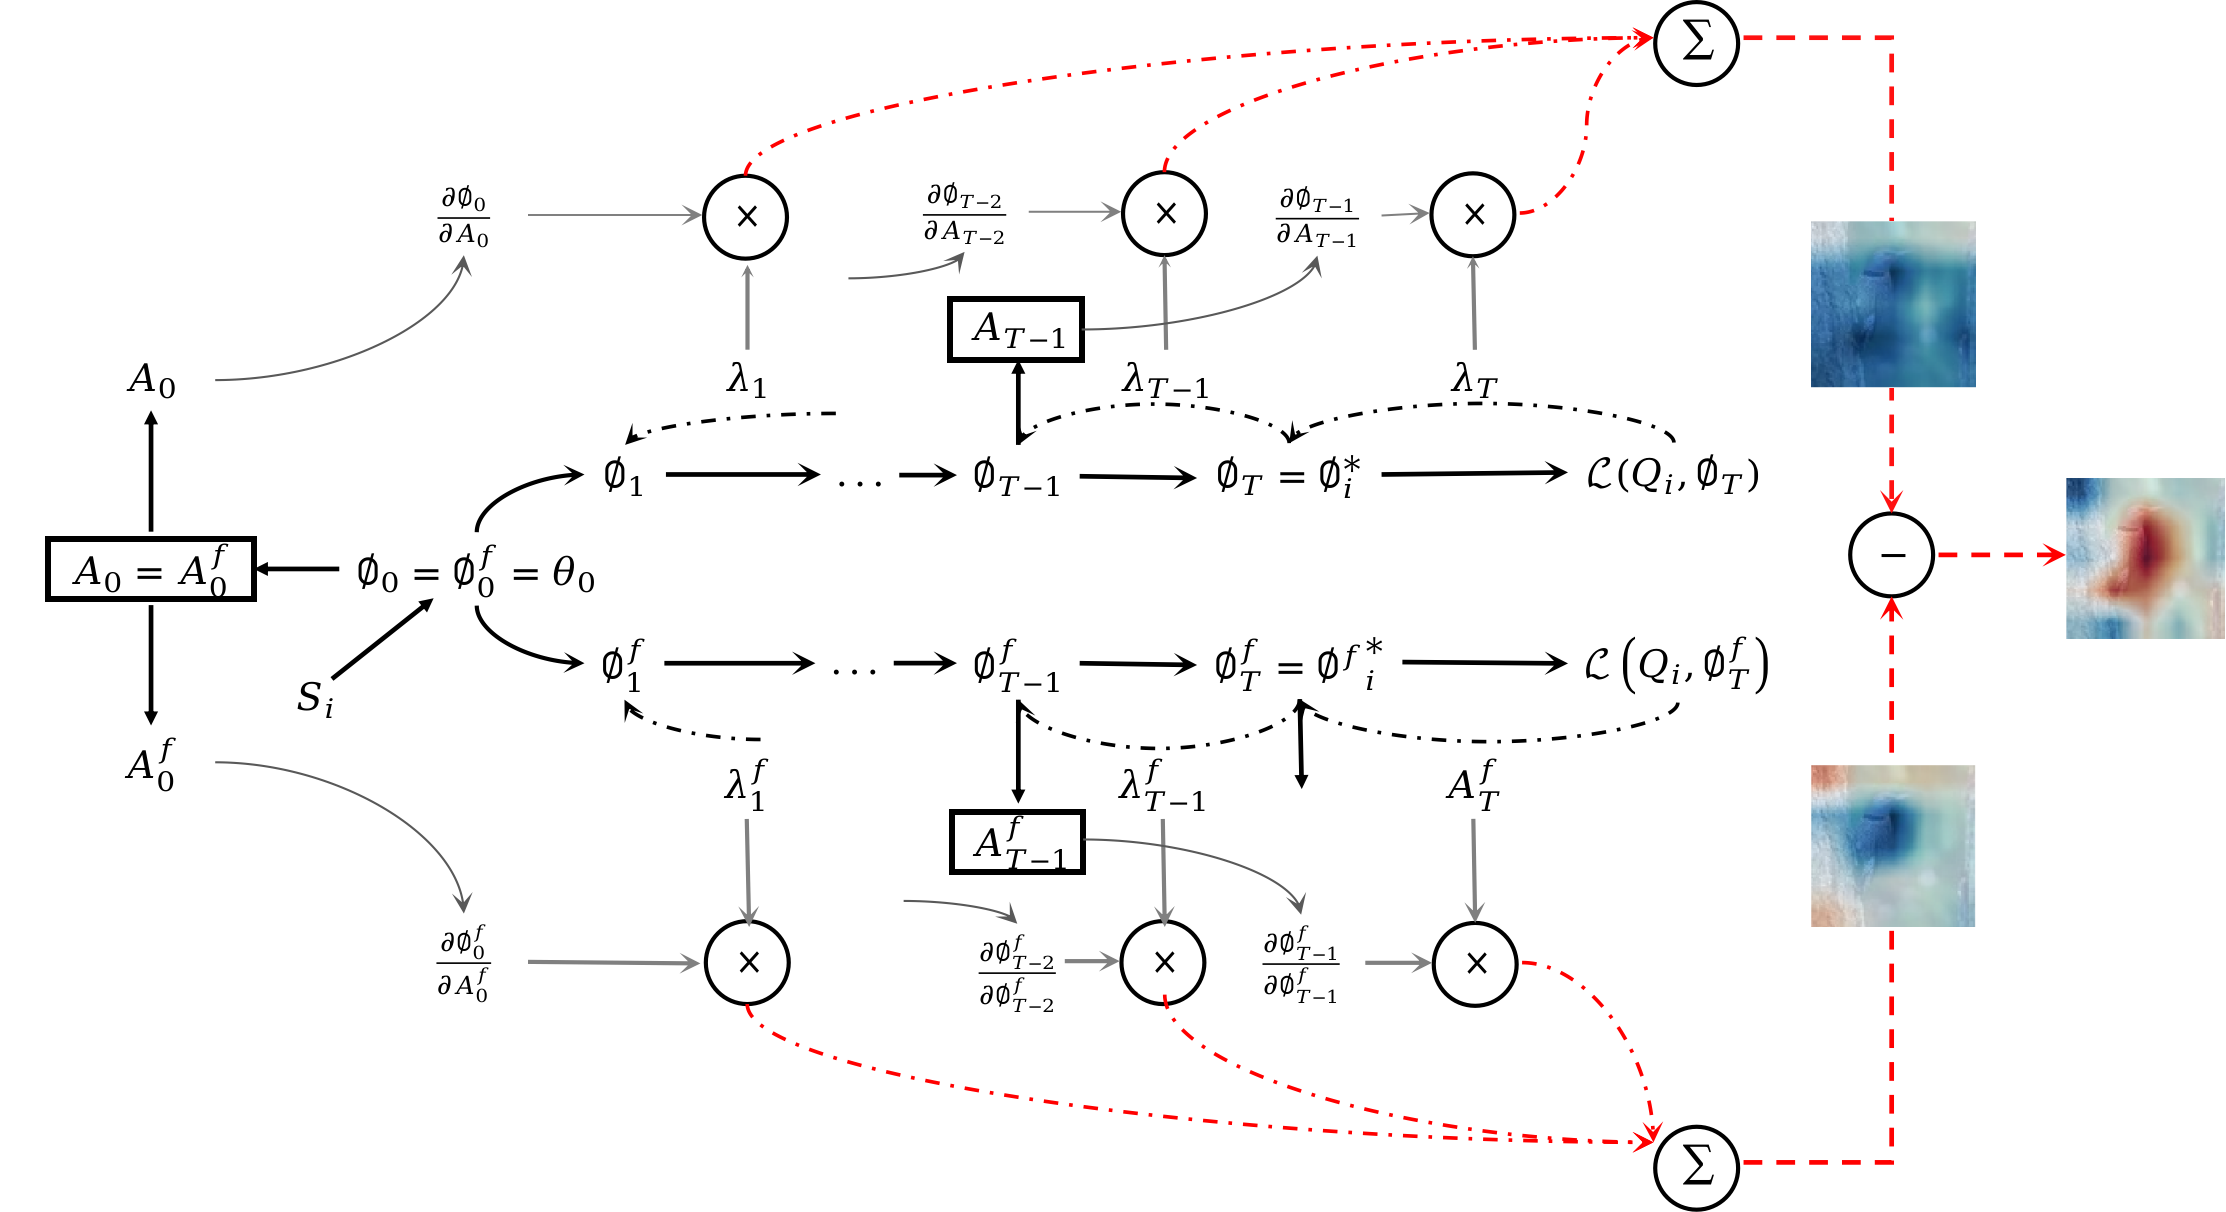
\includegraphics[width=0.5\linewidth]{figures/fama_pipeline.png}
    \caption{\fama pipeline. Two trajectories from $S_i$ (full adaptation, top; head-only/frozen-backbone, bottom) each get one backward adjoint pass computing $\{\lambda_t\}$; at every step $\lambda_t$ is projected onto the local feature map $A_{t-1}$ (Grad-CAM style), the $T$ local maps are accumulated per branch, and the two branch maps are subtracted into $\Phi_{\mathrm{FAMA}}$.}
    \label{fig:pipeline}
\end{figure}

\paragraph{Trajectory expansion.}
One inner-loop step has Jacobian
\begin{equation}
    \frac{\partial \phi_t}{\partial \phi_{t-1}} = I-\alpha H_{t-1},\qquad H_{t-1}:=\nabla^2_\phi \mathcal{L}(\phi_{t-1}, S_i).
    \label{eq:step_jacobian}
\end{equation}
Since $S_i$ is a shared \emph{input} to every step of \Cref{eq:inner_loop}, the chain rule sums its contribution over all $T$ steps:
\begin{equation}
    \frac{\partial\mathcal{L}(Q_i,\phi_T)}{\partial S_i} = -\sum_{t=1}^{T}\alpha\,\lambda_t\cdot\frac{\partial^2\mathcal{L}(\phi_{t-1},S_i)}{\partial\phi_{t-1}\partial S_i},\quad
    \lambda_t := \frac{\partial\mathcal{L}(Q_i,\phi_T)}{\partial\phi_t}.
    \label{eq:trajectory_expansion}
\end{equation}
Computing every $\lambda_t$ by literally unrolling and multiplying the $P\times P$ step-Jacobians of \Cref{eq:step_jacobian} is exactly the intractable BPTT case above.

\paragraph{Adjoint recursion.}
Instead, we treat $\{\lambda_t\}$ as the discrete-time adjoint (co-state) of Pontryagin's maximum principle \citep{pontryagin1962mathematical}: initialized at the trajectory endpoint and propagated \emph{backward} one Hessian-vector product (HVP) at a time,
\begin{equation}
    \lambda_T := \mathbb{E}_{Q_i}\!\big[\nabla_\phi\mathcal{L}(Q_i,\phi_T)\big],\quad
    \lambda_{t-1} = \lambda_t - \alpha H_{t-1}\lambda_t.
    \label{eq:adjoint_recursion}
\end{equation}
We prove by backward induction (\Cref{app:adjoint}) that this recursion computes $\lambda_t=\partial\mathbb{E}_{Q_i}[\mathcal{L}(Q_i,\phi_T)]/\partial\phi_t$ \emph{exactly} at every $t$ -- no linearization beyond \Cref{eq:inner_loop} itself, unlike neural-ODE adjoints that must also discretize a continuous system. Stability requires the standard non-expansiveness condition $\alpha\le 2/\lambda_{\max}(H_{t-1})$ (\Cref{app:adjoint}), satisfied by the fast-adaptation regime of Assumption~\ref{asm:fast_adaptation} for typical spectra. Each HVP is evaluated with Pearlmutter's double-backward trick \citep{pearlmutter1994fast}, $H_{t-1}\lambda_t=\nabla_{\phi_{t-1}}\langle\nabla_{\phi_{t-1}}\mathcal{L},\lambda_t\rangle$, at $\mathcal{O}(P)$ cost without materializing $H_{t-1}$, so the full backward pass costs $\mathcal{O}(TP)$.

\paragraph{Local attribution and CAM projection.}
Let $A_{t-1}:=f_{\phi_{t-1}^b}(S_i)\in F$ be the feature map at step $t{-}1$. Since $A_{t-1}$ is recomputed by a different backbone state at every $t$, no single global feature map exists for one chain-rule pass to flow through -- instead, at each $t$ we detach $A_{t-1}$ into a leaf variable (stop-gradient) and define a \emph{local} attribution
\begin{equation}
    \mathrm{Attr}_{t-1} := \frac{\partial}{\partial A_{t-1}}\Big[\lambda_t\!\cdot\!\nabla_\phi\mathcal{L}(\phi_{t-1},S_i)\Big],\ t=1,\dots,T,
    \label{eq:local_attr}
\end{equation}
which, since the backbone is formally frozen at this step, reduces to exactly the head/feature Hessian block $\partial^2\mathcal{L}/\partial\phi^h\partial A$. We turn $\mathrm{Attr}_{t-1}$ into a heatmap with the standard Grad-CAM recipe \citep{selvaraju2020grad} -- pool to channel weights, weight-and-sum, bilinearly upsample -- applied at every $t$, then accumulated along the trajectory:
\begin{equation}
    \Phi(x_k^S) := \sum_{t=1}^{T}\alpha\,\widehat{\mathrm{CAM}}_{t-1}(x_k^S).
    \label{eq:branch_saliency}
\end{equation}
Unlike Grad-CAM, we \emph{do not} apply ReLU: both the sign of help and the sign of harm are diagnostic, so $\widehat{\mathrm{CAM}}_{t-1}$ keeps its sign throughout. Running this for both branches and subtracting isolates the part of the signal attributable to the backbone actually moving:
\begin{equation}
    \boxed{\ \Phi_{\mathrm{FAMA}}(x_k^S) := \Phi_{\mathrm{full}}(x_k^S) - \Phi_{\mathrm{freeze}}(x_k^S).\ }
    \label{eq:fama_final}
\end{equation}
$\Phi_{\mathrm{freeze}}$ is a static feature-reuse baseline (constant backbone across all $t$), so \Cref{eq:fama_final} cancels whatever the branches attribute in common and keeps only the part caused by the backbone's own displacement -- the same quantity \Cref{prop:decomposition} identifies as $C_b$. Regions with $\Phi_{\mathrm{FAMA}}{>}0$ are where adaptation \emph{helped}; regions with $\Phi_{\mathrm{FAMA}}{<}0$ are where it \emph{hurt}. \Cref{alg:fama} summarizes the computation; since \Cref{eq:branch_saliency}'s upsampling assumes a convolutional feature grid, \fama as stated targets convolutional backbones (\Cref{sec:limitations}).

\begin{algorithm}[t]
\caption{\fama}
\label{alg:fama}
\footnotesize
\begin{algorithmic}[1]
\Require $\theta_0$, task $(S_i,Q_i)$, steps $T$, rate $\alpha$
\Ensure adaptation gain $\Delta M$, attribution map $\Phi_{\mathrm{FAMA}}$
\State $m \gets$ head mask of $\theta_0$ (last param.\ block)
\State roll out $\{\phi_t\}_{t=0}^T$ via \Cref{eq:inner_loop}; $\{\phi_t^f\}_{t=0}^T$ likewise but reset backbone params to $\theta_0^b$ after every step ($m$)
\State $\Delta M \gets$ bootstrap estimate of \Cref{eq:adaptation_gain} over $Q_i$
\For{branch $X \in \{\phi, \phi^f\}$}
    \State $\lambda_T \gets \mathbb{E}_{Q_i}[\nabla_\phi \mathcal{L}(Q_i, X_T)]$ \Comment{bootstrap}
    \For{$t = T, \dots, 1$}
        \State $\lambda_{t-1} \gets \lambda_t - \alpha\cdot\mathrm{HVP}(X_{t-1}, \lambda_t, S_i)$ \Comment{Eq.~\eqref{eq:adjoint_recursion}, Pearlmutter}
    \EndFor
    \State $\Phi_X \gets 0$
    \For{$t = 1, \dots, T$}
        \State $\Phi_X \mathrel{+}= \alpha \cdot \mathrm{GradCAM}(X_{t-1}, \lambda_t, S_i)$ \Comment{Eqs.~\eqref{eq:local_attr}--\eqref{eq:branch_saliency}, no ReLU}
    \EndFor
\EndFor
\State \Return $\Delta M$, $\ \Phi_{\mathrm{FAMA}} \gets \Phi_{\phi} - \Phi_{\phi^f}$
\end{algorithmic}
\end{algorithm}

\paragraph{Practical overhead.} Relative to one static Grad-CAM call (one forward, one backward, at $\phi_T$), \Cref{alg:fama} costs, per branch: $T$ inner-loop steps, $T$ HVPs, and $T$ local Grad-CAM projections -- each a fixed-size pass through the same backbone, independent of $P$. So the overhead is $\Theta(T)$ backbone evaluations with a small constant factor, not the quadratic-in-$P$ blowup literal BPTT would incur; this count is architectural, derived from \Cref{alg:fama}, not yet measured as wall-clock time (\Cref{sec:limitations}).
